% How to use writeLaTeX: 
%
% You edit the source code here on the left, and the preview on the
% right shows you the result within a few seconds.
%
% Bookmark this page and share the URL with your co-authors. They can
% edit at the same time!
%
% You can upload figures, bibliographies, custom classes and
% styles using the files menu.
%
%%%%%%%%%%%%%%%%%%%%%%%%%%%%%%%%%%%%%%%%%%%%%%%%%%%%%%%%%%%%%%%%%%%%%%

\documentclass[12pt,english,brazil]{article}
\usepackage{sbc-template}
\usepackage{adjustbox}
\usepackage{graphicx,url}
\usepackage{graphics}
\usepackage{color}
\usepackage{colortbl}
\usepackage[utf8]{inputenc}  
% Coloquei esse pacote para tamanho pequeno de fonte
\usepackage{scalefnt}
\usepackage{multirow}
\usepackage{subfigure}
\usepackage{multicol}
\usepackage{babel}
\babeltags{br = brazil, en = english}
\usepackage[T1]{fontenc}
\usepackage{xspace}
\usepackage{url}

\usepackage{xargs}
\usepackage[colorinlistoftodos,prependcaption,textsize=tiny]{todonotes}
\newcommandx{\ups}[2][1=]{\todo[linecolor=red,backgroundcolor=red!25,bordercolor=red,#1]{\tiny Gerson: #2}\xspace}
\newcommandx{\aham}[2][1=]{\todo[linecolor=yellow,backgroundcolor=yellow!25,bordercolor=yellow,#1]{\tiny Gui: #2}\xspace}
     
\sloppy

\title{Estudo de viabilidade do uso de Raspberry como servidor R-Shiny}

\author{Guilherme de Souza\inst{1}}


\address{Programa de Pós-Graduação em Computação \\Universidade Federal de Pelotas (UFPel)\\
  Caixa Postal 354 -- 96010.610 -- Pelotas -- RS -- Brazil
\nextinstitute
  Instituto de Matemática e Estatística (IME) -- Universidade de São Paulo (USP)\\
  Rua do Matão, 1010 -- São Paulo -- SP -- Brazil
  \email{\{gdsdsilva,gerson.cavalheiro\}@inf.ufpel.edu.br, gold@ime.usp.br}
}

\begin{document} 

\maketitle
    
\en
\begin{abstract}


\end{abstract}

\br
\begin{resumo} 


\end{resumo}



\section{Introdução}

A decisão economica sobre diferentes frentes por vezes passa pela análise de uma grande massa de dados. R é uma ferramenta que oferece grande potencial para manipulação e visualização de massas de dados. Shiny é um pacote para R que permite que servidores disponibilizem recursos para visualizações R.

R é uma ferramenta livre, existem outras, X e Y, que oferecem soluções semelhantes, porém, em um contexto proprietário. Este trabalho tem por objetivo avaliar o poder de escalabilidade de servidores web R, utilizando shiny.

O caso de estudo encaminhado considera o serviço WebShyda. São consideradas duas plataformas de suporte: um servidor com arquitetura convencional e um dispositivo de baixa capacidade (small board). O objetivo deste estudo é identificar componentes do sw, atualmente construído de forma monolítica, em microserviços. 

\section{Trabalhos Relacionados} \label{sec:TrabalhosRelacionados}
%RASCUNHOOOOOOO
%Referencias antigas quanto ao pq usar o raspberry (green computing)
\cite{Joao} propôs avaliar a substituição do hardware convencional por um hardware de baixo consumo que respeite o Service-Level-Agreement (SLA) e reduza o consumo de energia dos \textit{data centers}, assim tornando viável o uso de uma \textit{Small Board} em uma nuvem computacional.

Com isso, implementou a Raspbarry PI B+ como um nodo computacional de baixo consumo, realizando as adaptações necessárias para compatibilidade com a arquitetura ARM, precisando escolher um \textit{hypervision} adequado para tal. A nuvem era composta por 10 computadores de arquitetura x64, sendo nove deles nodos computacionais e um nodo de controle, em meio a essa composição a Raspberry vinha à acrescer como mais um nodo computacional.


A medição foi realizada através da execução do bechmark YCSB (\textit{Yahoo! Cloud Serving Benchmark}) que é especificamente desenvolvido para avaliar nuvens. Os resultados foram obtidos através da vazão de operações onde acabou por demonstrar um gargalo de processamento quando comparado ao nó de um baixo consumo. Porém a implementação da Rapberry PI B+ em uma nuvem, ainda sim é vantajosa, onde as características batam com as desempenhada pelo \textit{benchmark}.


Em \cite{PiConsumo} segue a mesma preocupação com o alto consumo de energia vindo das \textit{clouds}, porém até 2012, 10,82\% da população mantem assinatura de banda larga até, mantendo 770 milhões de gateways domeśtico ao redor do mundo. Tendo um consumo de 10W cada, gerando um consumo unitário de 6,7TWh ao ano o que soma em 0,03\% na energia consumida mundialmente. Levando em consideração que os maiores consumo ocorrem por parte de maquinas com um \textit{hardware} mais poderoso, ainda sim não se pode ignorar o consumo vindo por parte de tais dispositivos, pois 43\% dos mesmo se mantem ligados diariamente e muitas vezes ociosos, durante esse período de ociosidade, poderia vir desempenhar funções de pré-carregamento para usuario (ou seja, armazenamento em cache, pré-busca de conteúdo, execução de serviços locais).


A Raspberry PI vem sendo utilizada para inúmeras aplicações no qual fomenta o uso de tais aplicações com a visão em baixo consumo energético, com isso \cite{PiConsumo} apresenta o PowerPi um modelo de  potência concentrando-se no consumo de energia da Raspberry PI a fim de derivar novas possíveis estratégias de consumo de energia.

\section{WebSyhda}\label{sec:websyhda}

%RASCUNHOOOOOOOOO
Engenharia e gestão de recursos hídricos mantém uma grande dependência de séries hidrológicas. No entanto, o processamento destas séries é complexo, geralmente dependente de métodos numéricos para resolução, e é suscetível a erros quando feito de forma manualmente. Esses aspectos frequentemente dificultam a elaboração de projetos que depende da análise e estudo de séries hidrológicas. Com isso O Grupo de Pesquisa em Hidrologia e Modelagem Hidrológica em Bacias Hidrográficas/CNPq da UFPEL, propôs, desenvolveu e mantem O \emph{System of Hydrological Data Acquisition and Analysis} ou SYHDA \cite{syhda}.

A plataforma recentemente passou por uma migração para o modelo Web, onde encontra-se em constante desenvolvimento. É integralmente desenvolvida em R, com auxílio do RStudio e de inúmeras bibliotecas gratuitas de uso geral, uso específico para a hidrologia e de funcionalidades para ambiente Web. %li no cobalto

O WebSYHDA permite a importação de dados do Hidroweb/ANA\footnote{ANA: \url{https://dadosabertos.ana.gov.br}}, para dados de vazão, chuva e nível. Estes dados são reconhecidos pela plataforma de forma automática. Outras fontes de dados estão sendo implementadas na plataforma, como BDMEP/INMET\footnote{INMET: \url{https://portal.inmet.gov.br}} e dados oriundos de estações de monitoramento diversas com formatos definidos pelo usuário.

A plataforma em sua versão atual, conta com diversas funcionalidades, bem como: estatísticas descritivas, representações gráficas, testes não paramétricos, consistência de dados de chuva, análise de frequência local e análise de frequência regional. Os resultados serão estruturados de forma dinâmica, assim permitindo o manuseio pelo usuário final, permitindo ainda a possibilidade de exportação e salvar o estado atual do projeto. 

\section{Metodologia} \label{sec:metodologia}

Visto que a demanda de serviços \textit{web} ocupa a maior parte das aplicações na nuvem, maiores são os esforços para otimização das aplicações para um menor consumo de requisitos e rede. 

Dito isso, para este trabalho fizemos uso de uma aplicação real, o WebSyhda como mecanismo de teste, que permitiu equiparar \emph{hardware} de arquitetura x64 com a \emph{smallboard} selecionado, Raspberry PI 3, dada a eficiência apresentada pelo dispositivo em trabalhos anteriores e a capacidade de atender cenários de demanda \emph{web} \cite{silva2019estudo}.

Para simulação de carga fizemos uso da ferramenta \emph{Shinycannon}, a qual nos permite simular usuários simultaneos realizando ações no aplicativo. Assim atendendo nossas exigências em quantativar numero de usuários suportados e latência do aplicativo.



\subsection{Linguagem R} \label{sec:R}

R é uma linguagem e ambiente com foco em computação estatística e gráficos. Assim, R permite desenvolver e publicar gráficos bem projetados \cite{whatR}, semelhantemente a C/C++ e outras linguagens disponíveis no mercado, R também permite o desenvolvimento por meio de módulos, mas ainda se tratando de uma unica e grande aplicação.
%Colocar sobre a forma de escalabilidade do R aqui?!

Com isso vale ressaltar que R é uma aplicação de thread único, o que significa que um aplicativo não pode atender a dois usuários diferentes precisamente ao mesmo tempo, Figura ~\ref{singleThreads}. Em muitas aplicações isso não é um problema, porque a maioria dos cálculos leva apenas dezenas ou centenas de milissegundos. Como resultado, um único processo R geralmente pode atender de 5 a 30 solicitações por segundo \cite{ShinyappsEscalabilidade}. 

\begin{figure}[htbp]
  \centering 
  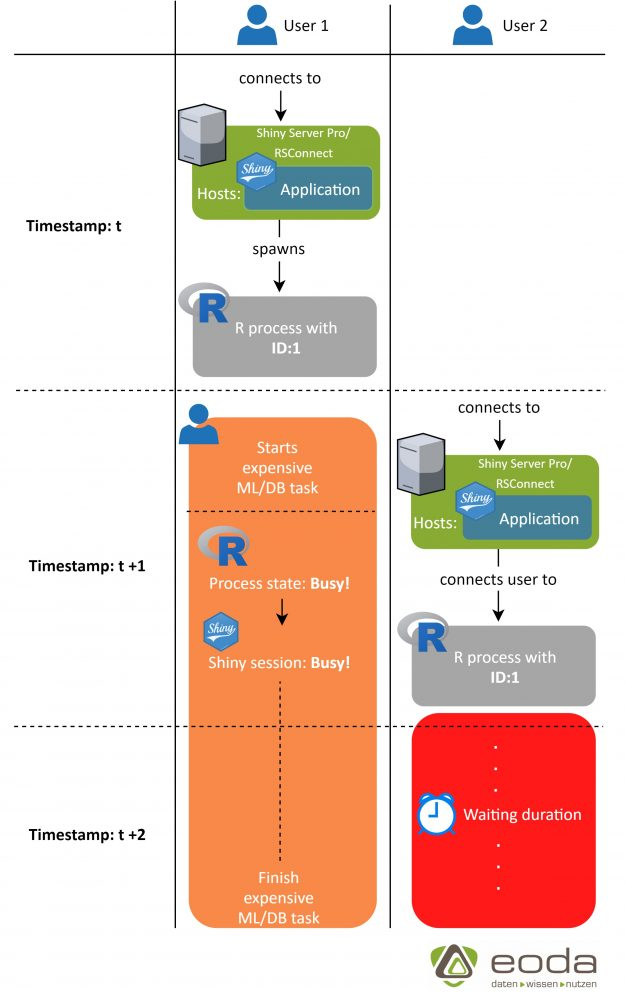
\includegraphics[scale=.4]{figures/single_threads.jpg}
  \caption{Exemplo de uma execução sequencial \cite{singleThreads}}
  \label{singleThreads}
\end{figure}

\subsection{Shiny} \label{sec:Shiny}

Para o desenvolvimento de aplicativos \emph{web} fazendo uso da linguagem R, a Rstudio mantém o pacote \emph{Shiny}\footnote{Shiny: \url{https://shiny.rstudio.com}}. Um pacote R que facilita a construção de aplicativos interativos. Permitindo hospedar aplicativos independentes em uma página da web ou incorporá-los em documentos R Markdown ou construir painéis. 

Assim, torna-se possivel apresentar gráficos dinamicos e iterativos por meio de pacotes como, ggvis\footnote{ggvis: \url{https://ggvis.rstudio.com/}}, ggiraph\footnote{ggiraph: \url{https://davidgohel.github.io/ggiraph/}}, plotly\footnote{plotly: \url{https://plotly.com/}} entre outros mantidos pela RStudio ou pela comunidade. Permitindo ainda, estender os aplicativos \emph{Shiny} com temas CSS (\emph{Cascading Style Sheets}), \emph{htmlwidgets} e ações JS (\emph{JavaScript}).

\subsection{Shinycannon} \label{sec:Shinycannon}

\textit{Shinycannon}\footnote{Shinycannon: \url{https://github.com/rstudio/shinycannon}} é uma ferramenta de linha de comando que possibilita testes de carga em aplicativos R. De forma a permitir aos desenvolvedores analisarem a escalabilidade de seu aplicativo simulando de um a n usuários simultaneos.

A Ferramenta acompanha o pacote \textit{shinyloadtest}\footnote{Shinyloadtest: \url{https://rstudio.github.io/shinyloadtest/}}, mantido pela própria Rstudio. O pacote é responsavel por gerar uma gravação de uma sessão de usuário, essas sessões podem ser criadas pensando no uso tipico do aplicativo desenvolvido\cite{shinyloadtest}. A sessão é criada de forma manual, após a iniciação do pacote o tester executa a interação com o aplicativo de forma natual, assim como um usuário comum. Ao terminar seu uso basta fechar a aplicação para que o pacote encerre a gravação da sessão.

Com isso, por sua vez, a \textit{Shinycannon} permite a criação de trabalhadores, que são os usuários simulados, podendo criar tantos quantos necessarios para execução dos testes. Assim para execução dos teste devemos definir o numero de trablhadores e o tempo total da sessão que será executada pelos mesmos. 

Em suma, a \textit{Shinycannon} replica os passos da gravação criada pelo pacote \textit{Shinyloadtest} entre seus trabalhadores (usuários), fazendo com que cada trabalhador execute simultaneamente a mesma sessão durante o tempo definido pelo desenvolvedor.

\subsection{Hardware}\label{sec:Hardware}
Com a popularização do uso de serviços providos pela computação em nuvem, o consumo energético dos data centers também aumentou, chegando a 270 TWh em 2012 \cite{VanHeddeghem:2014:TWI:2657027.2657141}, estimando chegar a mais de 2\% do consumo da energia mundial apos 2020 \cite{energy}.  Buscando alternativas de evitar esse alto consumo energético das máquinas convencionais utilizadas em data centers, o uso de dispositivos com arquitetura ARM, que possuem baixo consumo energético, são uma das estratégias possíveis.

Assim, o dispositivo de teste escolhido foi a \emph{smallboard} Raspberry PI3, dada sua arquitetura ARM aberta, comunidade participativa em inumeros projetos alem de sua alta disponbilidade no mercado. As especificacoes do device podem ser observadas na Tabela ~\ref{tab:especificacao}.

\begin{table}[!h]
    \centering
    \caption{Especifícação de \textit{hardware} do dispositivo, segundo o fabricante~\cite{fundation2015raspberry}.}
    \label{tab:especificacao}
    \begin{tabular}{c|c}
    \hline
    \textbf{Espesificações}                                           & \multicolumn{1}{l}{\textbf{Raspeberry PI 3}}                             \\ \hline
    Processador                                                       & \begin{tabular}[c]{@{}c@{}}BCM2837 64Bit\\ Quad Core 1.2GHz\end{tabular} \\ \hline
    Arquitetura                                                       & ARMv8                                                                    \\ \hline
    RAM                                                               & 1GB SDRAM 400MHz                                                         \\ \hline
    Armazenamento                                                     & Micro SD                                                                 \\ \hline
    USB 2.0                                                           & 4 Portas USB                                                             \\ \hline
    \begin{tabular}[c]{@{}c@{}}Máxima corrente/\\ Tensão\end{tabular} & \begin{tabular}[c]{@{}c@{}}2,4A/\\ 5V\end{tabular}                       \\ \hline
    GPIO                                                              & 40 Pins                                                                  \\ \hline
    \end{tabular}
    \end{table}
    
Para comparativo de desempenho, utilizou-se um dispositivo de arquitetura x64.
O \textit{server} selecionado para tal comparativo foi o HP ----------------- \cite{}, suas especificações se encontrão presente na Tabela \ref{tab:especificacaoserver}, informações obtidas através do comando \textit{dmidecode}, o qual apresenta todas informações disponíveis sobre o dispositivo, possibilitando uma pesquisa mais especifica dentro dele atribuindo ao comando \textit{dmidecode --type} concatenado com uma chave da tabela de representação do comando, como a chave quatro, nos demonstrará todas especificações do processador e assim por diante.

\begin{table}[!h]
    \centering
    \caption{Especifícação de \textit{hardware} do \textit{server}.}
    \label{tab:especificacaoDesktop}
    \begin{tabular}{cc}
    \hline
    \multicolumn{1}{c|}{\textbf{Espesificações}}                                           & \textit{\textbf{Desktop}}                                                                   \\ \hline
    \multicolumn{1}{c|}{Processador}                                                       & \begin{tabular}[c]{@{}c@{}}8x Intel(R) Core(TM) i7-3370\\ CPU @ 3.40GHz 64Bits\end{tabular} \\ \hline
    \multicolumn{1}{c|}{Arquitetura}                                                       & x64                                                                                     \\ \hline
    \multicolumn{1}{c|}{RAM}                                                               & XGB X.xxxMHz                                                                                \\ \hline
    \multicolumn{1}{c|}{Armazenamento}                                                     & HD                                                                                         \\ \hline
    \multicolumn{1}{c|}{USB 2.0}                                                           & 4 Portas USB                                                                                \\ \hline
    USB 3.0                                                                                & 2 Portas USB                                                                                \\ \hline
    \multicolumn{1}{c|}{\begin{tabular}[c]{@{}c@{}}Máxima corrente/\\ Tensão\end{tabular}} & ---/---                                                                               \\ \hline
    \end{tabular}
    \end{table}

\subsection{Metodologia dos Testes}\label{sec:MetodologiaDosTestes}
A fim de testar o aplicativo no seu estágio atual de desenvolvimento e também encontrar cargas próximas ao limite da Raspberry PI, consideramos a documentação como base, onde a mesma demonstra qual seria aproximadamente o limite de tempo de resposta do aplicativo dada a quantidade de usuários \cite{documentShiny}.


%Em um primeiro momento, analisamos o uso mais comum do sw, ou seja, seu uso diário por engenheiros hídricos, a Figura ~\ref{usoWebSyhda} demonstra o conjunto de ações tomada dentro do aplicativo. Com isso utilizamos o pacote \emph{shinyloadtest}, assim permitindo a gravação deste conjunto de passos. 
Em um primeiro momento, buscou-se um teste que fosse característico de um fluxo típico de um usuário, fazendo uso de várias técnicas empregadas em diversas análises hidrológicas, porém com foco em tarefas que requerem maior processamento. Optou-se por utilizar o módulo de Análise de Frequência Regional para o teste, visto que o mesmo atende ao critério de uso anterior, assim como a exigência de múltiplos arquivos para computar os resultados. A Figura ~\ref{usoWebSyhda} demonstra o conjunto de ações tomada dentro do aplicativo. Com isso utilizamos o pacote \emph{shinyloadtest}, assim permitindo a gravação deste conjunto de passos. 

\begin{figure}[htbp]
  \centering 
  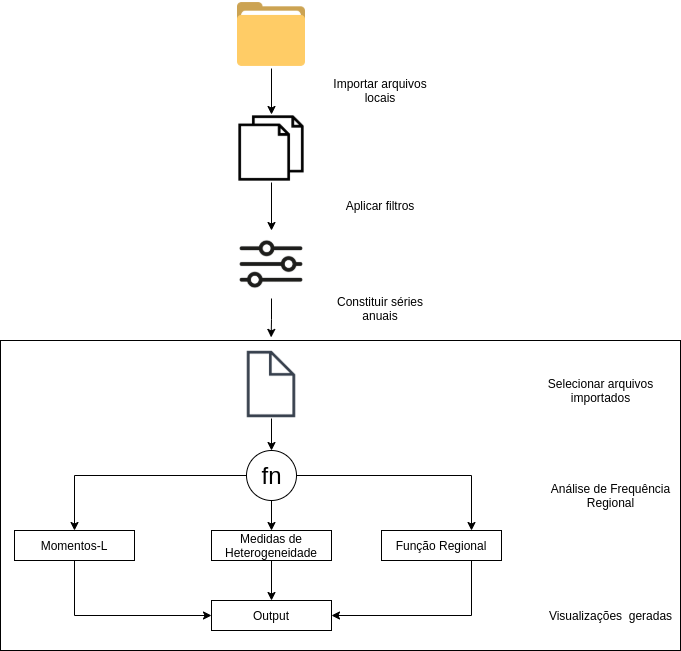
\includegraphics[scale=.4]{paperWSCAD2021/figures/useWebSyhdaDrawio.png}
  \caption{Exemplo dos passos seguido pelo usuário}
  \label{usoWebSyhda}
\end{figure}

Inicialmente partimos com um conjunto de execuções teste afim de entender o simulador e as possibilidades fornecidas por ele. Seguindo as indicações da documentação e observando o tempo comum de trabalho de um usuário do \emph{WebSyhda}, concluímos que %mudar isso
dois minutos representa mais de uma execução do conjunto de passos propostos, o que demonstra uma maior realidade de uso do aplicativo. Assim sendo, utilizamos dois minutos como limite de tempo de execução da ferramenta para nossa coleta.



%Nesses passos 10 arquivos foram utilizandos ... onde realiza ....

De forma semelhante, realizamos o aumento da carga parcialmente iniciando em um único trabalhador, logo após passamos a incrementar como demonstrado pela tabela ~\ref{tab:workers}. Para definição do limite de trabalhadores suportados, seguimos a documentação disponibilizada pela ferramenta, onde a mesma define que se aplicativos continuar sua execução muito tempo após a finalização do script, naturalmente ocasionam em respostas finais mais demoradas para o usuário final, assim, demonstrando a necessidade de recodificação do aplicativo ou o aumento de requisitos de \emph{hardware}. Todo o roteiro de testes e os arquivos gerados aqui apresentados, estão disponíveis no GitHub\footnote{GitHub: \url{https://github.com/SouzaGuilherme/research_PI3_R-Shiny-server}}.

\begin{table}[htbp]
\centering
\label{tab:workers}
\caption{Número de trabalhadores e tempo de simulação utilizados nos testes}
\begin{tabular}{c|c|cc}
\hline
\multicolumn{2}{c|}{\textbf{Servidor HP}} & \multicolumn{2}{c}{\textbf{Raspberry PI 3}}             \\ \hline
Trabalhadores     & Tempo                 & \multicolumn{1}{c|}{Trabalhadores} & Tempo              \\ \hline
1                 & \multirow{3}{*}{2}    & \multicolumn{1}{c|}{1}             & \multirow{3}{*}{2} \\ \cline{1-1} \cline{3-3}
10                &                       & \multicolumn{1}{c|}{10}            &                    \\ \cline{1-1} \cline{3-3}
20                &                       & \multicolumn{1}{c|}{20}            &                    \\ \hline
\end{tabular}
\end{table}

\section{Resultados} \label{sec:Resultados}
Após a análise dos resultados obtidos a partir da execução do simulador nos cenários criados, focamos nos resultados de latência máxima de \emph{websocket}, ou seja, tempo de cálculo. Ressaltamos que os resultados aqui apresentados consideram os cenários e o estágio do aplicativo no momento de proposta deste trabalho. Para uma melhor visualização dos resultados, o próprio simulador desconsidera o tempo de aquecimento dos trabalhadores. Todos os resultados, estão disponíveis para consulta no GitHub\footnote{GitHub: \url{https://github.com/SouzaGuilherme/research_PI3_R-Shiny-server}} junto aos fontes.

 

\section{Conclusão} \label{sec:conlusao}



\bibliographystyle{sbc}
\bibliography{sbc-template}

\end{document}
